\section{RQ1 (Scope): On Which Systems Does a Pooled Advantage Hold?}
\label{sec:rq1}

\Cref{tab:main} gives every method's accuracy on every subsystem; cells with coverage below 1 are marked, and randomized methods are averaged over three seeds.
The familiar picture of a pooled leaderboard appears only after averaging over columns.
Within a family the best method changes from column to column: on RE1 it is \baro on two applications and \cdmin on the third; on \petshop it is a shipped baseline in all four scenarios, but not always the same one.
RQ1 asks how often a comparison that a pooled leaderboard would report holds on each of the subsystems behind it.

\begin{table}[t]
\caption{Accuracy (\acc; \openrca: official partial score) of every method on every subsystem, over all cases (invalid outputs score 0). $^\dagger$: coverage below 1. Bold: best in column. Each panel lists the methods that run on at least one of its families (\cref{sec:design-methods}); --: the method does not run on that release. \rcd and \causalrca: mean of three seeds (\petshop's own \rcd: one run).}
\label{tab:main}
\footnotesize
\setlength{\tabcolsep}{4pt}
\centering
\begin{tabular*}{\textwidth}{@{\extracolsep{\fill}}lrrrrrr@{}}
\toprule
 & \multicolumn{3}{c}{RCAEval RE1} & \multicolumn{3}{c}{RCAEval RE2} \\
\cmidrule(lr){2-4} \cmidrule(lr){5-7}
$n$ & 125 & 125 & 125 & 90 & 90 & 90 \\
Method & OB & SS & TT & OB & SS & TT \\
\midrule
\multicolumn{7}{@{}l}{\textit{Published methods}} \\
BARO & {\bfseries 0.736} & 0.848 & {\bfseries 0.560} & 0.144 & 0.067 & 0.667 \\
CIRCA & 0.672 & 0.704 & 0.328 & 0.667 & 0.778 & 0.544 \\
$\epsilon$-Diagnosis & 0.032 & 0.144 & 0.000 & 0.033 & 0.156 & 0.000 \\
RCD & 0.541 & 0.389 & 0.088 & -- & -- & -- \\
CausalRCA & 0.616 & 0.176 & 0.136 & 0.207 & 0.148 & 0.207$^\dagger$ \\
SimpleRCA & -- & -- & -- & 0.467 & 0.244 & {\bfseries 0.800} \\
TraceRCA & -- & -- & -- & 0.100 & -- & 0.533$^\dagger$ \\
MicroRank & -- & -- & -- & 0.000 & -- & 0.122$^\dagger$ \\
BARO (multi-source) & -- & -- & -- & 0.167 & 0.067 & 0.689$^\dagger$ \\
\midrule
\multicolumn{7}{@{}l}{\textit{Probes}} \\
max-$|Z|$ & 0.504 & 0.744 & 0.424 & {\bfseries 0.778} & 0.844 & 0.411 \\
Alert-count & 0.392 & 0.376 & 0.048 & 0.211 & 0.389 & 0.211 \\
CD-1min & 0.728 & {\bfseries 0.928} & 0.280 & 0.733 & {\bfseries 0.944} & 0.789 \\
\bottomrule
\end{tabular*}
\par\medskip
\begin{tabular*}{\textwidth}{@{\extracolsep{\fill}}lrrrrrrrr@{}}
\toprule
 & \multicolumn{4}{c}{OpenRCA} & \multicolumn{4}{c}{PetShop} \\
\cmidrule(lr){2-5} \cmidrule(lr){6-9}
$n$ & 136 & 70 & 78 & 51 & 26 & 26 & 8 & 8 \\
Method & Bank & Mkt-1 & Mkt-2 & Tel & High & Low & Tmp-1 & Tmp-2 \\
\midrule
\multicolumn{9}{@{}l}{\textit{Published methods}} \\
BARO & 0.160 & 0.057 & 0.106 & 0.183 & 0.154 & 0.154 & 0.250 & 0.250 \\
CIRCA & -- & -- & -- & -- & 0.269 & 0.385 & 0.500 & 0.625 \\
$\epsilon$-Diagnosis & 0.036 & 0.038 & 0.044 & 0.046$^\dagger$ & 0.000$^\dagger$ & 0.000$^\dagger$ & 0.000$^\dagger$ & 0.125 \\
RCD & 0.089 & 0.051$^\dagger$ & 0.066$^\dagger$ & 0.193$^\dagger$ & 0.000 & 0.346 & 0.625 & 0.375 \\
Counterfactual & -- & -- & -- & -- & 0.308 & 0.154 & 0.125 & 0.250 \\
\midrule
\multicolumn{9}{@{}l}{\textit{Probes}} \\
max-$|Z|$ & 0.127 & 0.161 & {\bfseries 0.200} & 0.232 & 0.077 & 0.192 & 0.375 & 0.375 \\
Alert-count & {\bfseries 0.172} & 0.144 & 0.197 & {\bfseries 0.242} & 0.038 & 0.000 & 0.000 & 0.250 \\
CD-1min & 0.165$^\dagger$ & {\bfseries 0.161} & 0.192 & 0.163$^\dagger$ & 0.000 & 0.038 & 0.125 & 0.125 \\
\midrule
\multicolumn{9}{@{}l}{\textit{Shipped baselines}} \\
Traversal & -- & -- & -- & -- & 0.385$^\dagger$ & {\bfseries 0.577$^\dagger$} & 0.625 & {\bfseries 0.875} \\
Ranked correlation & -- & -- & -- & -- & {\bfseries 0.731$^\dagger$} & {\bfseries 0.577$^\dagger$} & {\bfseries 0.750} & 0.500 \\
Random walk & -- & -- & -- & -- & 0.000$^\dagger$ & 0.000$^\dagger$ & 0.125 & 0.000 \\
\bottomrule
\end{tabular*}

\end{table}

\subsection{Comparisons Between Published Methods}
\label{sec:rq1-pub}

\Cref{fig:forest} shows every comparison between two published methods that a family allows, with each subsystem's difference and its CI.
Two families carry comparisons that exist in the literature, RE1 and \petshop; the \openrca comparisons are our construction (\cref{sec:design-bench}) and are reported separately below.
Of the \NAudPubPairs pairs on RE1 and \petshop, \NAudPubRev reverse on at least one subsystem and \NAudPubRevCI do so with CI support; with the \NOpenrcaPubPairs \openrca pairs the counts are \NMainPubRev and \NMainPubRevCI of \NMainPubPairs.
\NAudPubEdiagPairs of the \NAudPubPairs pairs involve \ediag, which is never more accurate than the other method on any subsystem, so their stability is expected, and none of them reverses.
Dropping the two \petshop scenarios with 8 cases leaves \NAudPubRevNmin reversing pairs, \NAudPubRevCINmin with CI support, and at a Bonferroni-adjusted level \NBonfRevCI CI-supported reversal remains (\cref{sec:threats}).
Within a benchmark, then, a pooled lead between published methods mostly holds on every subsystem, and the exceptions are on \petshop; the rest of this section asks what the lead says beyond the subsystems it was computed on.
The reversing pairs are those whose pooled margin is small next to the spread of their subsystem differences (grey rows in \cref{fig:forest}); the split is partly definitional, and we use it only to read the figure.

\begin{figure}[t]
\centering
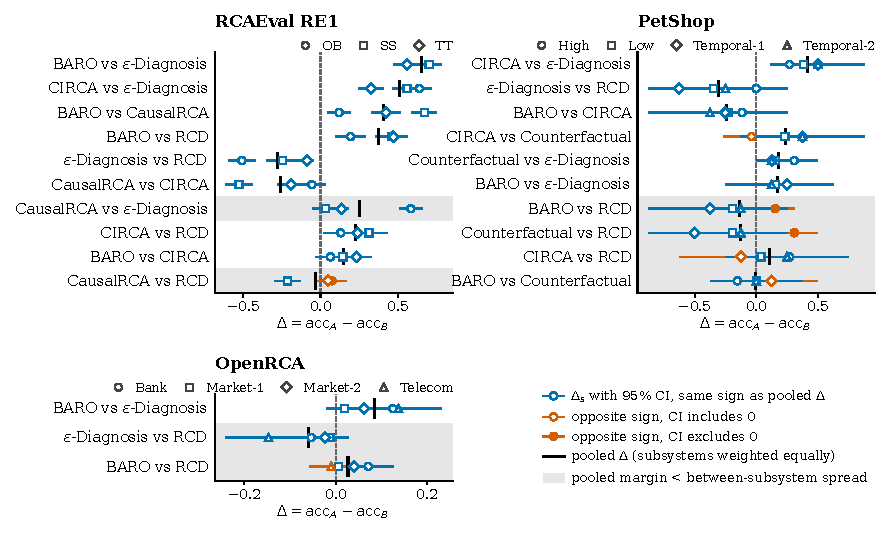
\includegraphics[width=\textwidth]{figures/fig1_forest.pdf}
\caption{Comparisons between published methods, by family. Each row is a pair $A$ vs $B$; markers are subsystem differences $\Delta_s$ with 95\% bootstrap CIs, the vertical tick is the pooled difference (subsystems weighted equally). Orange markers have the opposite sign of the pooled difference (filled: CI excludes 0). Grey rows: pairs whose pooled margin is smaller than the between-subsystem spread of $\Delta_s$.}
\label{fig:forest}
\end{figure}

\textbf{RCAEval RE1.}
Of \NReOnePubPairs pairs, \NReOnePubRev reverses, without CI support.
\baro leads each of the other four published methods on all three applications, with pooled margins from \ReOneBaroMinMargin to \ReOneBaroMaxMargin.
The one unstable pair is \causalrca vs \rcd: its pooled difference is \ReOneCrRcdPooled \ReOneCrRcdPooledCI, made of \ReOneCrRcdOB on OB, \ReOneCrRcdSS on SS, and \ReOneCrRcdTT on TT; both methods are randomized, and the pooled sign itself changes with the seed (\ReOneCrRcdSeedZero, \ReOneCrRcdSeedOne, \ReOneCrRcdSeedTwo).
This is RE1 under the reference configuration; on the files as shipped it is less stable (\cref{sec:rq2}).

\textbf{OpenRCA.}
These results measure each method together with our answer wrapper and the official scoring rule; no published paper compares these methods on \openrca, and they are not an audit of its agent leaderboard.
Under the wrapper, the three methods order as \baro (\OpenrcaBaroMean), \rcd (\OpenrcaRcdMean), \ediag (\OpenrcaEdiagMean).
\baro's lead over \rcd is \OpenrcaBaroRcdPooled \OpenrcaBaroRcdPooledCI, but Telecom reverses it (\OpenrcaBaroRcdTel \OpenrcaBaroRcdTelCI); the reversal rests on a few queries, and \OpenrcaBaroRcdSeedsWithRev of the three \rcd seeds show a reversal, on different subsystems.

\textbf{PetShop.}
The published methods are least stable here: \NPetshopPubRev of \NPetshopPubPairs pairs reverse, \NPetshopPubRevCI with CI support.
Both CI-supported reversals come from one cell: \rcd scores \PetshopRcdHighHits of \PetshopHighN on the high-traffic scenario, so \baro (\PetshopBaroRcdHigh \PetshopBaroRcdHighCI) and \cfa (\PetshopCfaRcdHigh \PetshopCfaRcdHighCI) beat it there while trailing it on pooled accuracy, with pooled CIs that include zero.
The two temporal scenarios have 8 cases each; keeping only the two scenarios with at least 25 cases leaves \PetshopPubRevNmin reversing pairs, \PetshopPubRevCINmin with CI support.

\subsection{Same Applications, Second Release}
\label{sec:rq1-release}

RE2 is a second, independently collected release of RE1's three applications, with new fault instances, a sixth fault type, and added logs and traces.
Its metric tables are also sampled differently (\ReTwoRows rows per case against \ReOneSSRows on RE1-SS) and record more metric kinds per service (\ReTwoOBCols columns on OB against \ReOneOBCols on RE1).
The four published methods that use metrics only (\baro, \circa, \ediag, \causalrca) run with the same implementations on both releases.
If a pooled RE1 lead were a property of the method and the application, it should carry over.
A release differs from its predecessor in collection as well as in faults, so what this section tests is carry-over between two releases of the same applications, not between systems.
Of the \NCrossPub application-level comparisons available in both releases (\cref{tab:release}), \NCrossPubAgree keep their sign and \NCrossPubCIopp have CIs on opposite sides of zero.
Both of the latter are on Sock Shop: \baro vs \circa goes from \CrossBaroCircaSSOne \CrossBaroCircaSSOneCI to \CrossBaroCircaSSTwo \CrossBaroCircaSSTwoCI, and \baro vs \causalrca from \CrossBaroCrSSOne to \CrossBaroCrSSTwo \CrossBaroCrSSTwoCI.
Restricting RE2 to RE1's five fault types leaves the count at \NCrossPubAgreeReOneFaults of \NCrossPub, so the added fault type alone does not explain the change; the released data do not allow the other differences between the releases to be separated.
Within RE2 itself, \NReTwoPubRev of \NReTwoPubPairs published pairs reverse across the three applications (\NReTwoPubRevCI with CI support).

The largest change between the releases is \baro's.
Its accuracy falls from \BaroAccReOneOB to \BaroAccReTwoOB on OB and from \BaroAccReOneSS to \BaroAccReTwoSS on SS, and a drop of this size calls for the checks of RQ2 before it is read as a property of the method.
It passes them: the ranking is not the input column order, every case has a valid output, and the root cause is still among \baro's first three candidates in \BaroReTwoOBAccThree of the OB cases and \BaroReTwoSSAccThree of the SS cases.
What changes is the first position.
RE2's reduced table adds disk I/O and socket metrics for every service, which RE1's tables do not contain, and \baro ranks the disk I/O of the application's database first in \BaroReTwoOBTopMetricN of the 90 OB cases and \BaroReTwoSSTopMetricN of the 90 SS cases, whatever the injected fault.
\citet{fang2025simplerca} report top-1 accuracies of 0.14 on both applications for their own \baro baseline on RE2, which places the drop in the release rather than in our runs.
A method's lead can thus depend on which metric kinds a release records, a part of a score's provenance that neither a leaderboard nor a per-system table states.

\begin{table}[t]
\caption{Same application, two releases: subsystem differences $\Delta_s$ ($A$ minus $B$) between published methods on RE1 and RE2. Bold: the two releases' 95\% CIs lie on opposite sides of zero.}
\label{tab:release}
\small
\setlength{\tabcolsep}{5pt}
\begin{tabular}{@{}lrrrrrr@{}}
\toprule
 & \multicolumn{2}{c}{Online Boutique} & \multicolumn{2}{c}{Sock Shop} & \multicolumn{2}{c}{Train Ticket} \\
\cmidrule(lr){2-3} \cmidrule(lr){4-5} \cmidrule(lr){6-7}
Pair $A$ vs $B$ & RE1 & RE2 & RE1 & RE2 & RE1 & RE2 \\
\midrule
BARO vs CausalRCA & +0.120 & $-$0.063 & {\bfseries +0.672} & {\bfseries $-$0.081} & +0.424 & +0.459 \\
BARO vs CIRCA & +0.064 & $-$0.522 & {\bfseries +0.144} & {\bfseries $-$0.711} & +0.232 & +0.122 \\
BARO vs $\epsilon$-Diagnosis & +0.704 & +0.111 & +0.704 & $-$0.089 & +0.560 & +0.667 \\
CausalRCA vs CIRCA & $-$0.056 & $-$0.459 & $-$0.528 & $-$0.630 & $-$0.192 & $-$0.337 \\
CausalRCA vs $\epsilon$-Diagnosis & +0.584 & +0.174 & +0.032 & $-$0.007 & +0.136 & +0.207 \\
CIRCA vs $\epsilon$-Diagnosis & +0.640 & +0.633 & +0.560 & +0.622 & +0.328 & +0.544 \\
\bottomrule
\end{tabular}

\end{table}

\subsection{Choosing a Method for an Unseen Subsystem}
\label{sec:rq1-heldout}

A practitioner choosing a method for a new system has only the other subsystems to go by.
Holding out each of the 11 subsystems in turn and ranking the published methods of its family on the remaining ones gives \HNDec adjacent-pair decisions.
In \HErr of them the higher-ranked method is less accurate on the held-out subsystem (\HStrict with a CI excluding zero), and \HTies further decisions are ties.
A ranking drawn at random would err in half of the \HNonTie non-tied decisions, \HRandErr; the pooled ranking is informative, and the question is where it is not.
\Cref{tab:regret} gives the cost of such a choice as regret.
The pooled winner chosen without the held-out subsystem has positive regret on \LosoRegPubN of the \LosoRegPubOf subsystems (up to \LosoRegPubMax), and with probes and shipped baselines on \LosoRegAllN of \LosoRegAllOf (up to \LosoRegAllMax).
For comparison, choosing a published method at random has an expected regret of \RegRandReOne on RE1, \RegRandOpenrca on \openrca, and \RegRandPetshop on \petshop, against mean regrets of \RegWinnerMeanReOne, \RegWinnerMeanOpenrca, and \RegWinnerMeanPetshop for the pooled winner.
The pooled winner is a far better default than a random choice; its cost is concentrated on particular subsystems.
The largest costs are concrete: on RE2, \circa has the highest pooled accuracy (\RegReTwoWinnerPooled) but scores \RegReTwoTTwinner on Train Ticket against \simplerca's \RegReTwoTTbest; on \petshop the pooled winner \circa trails another published method on the high-traffic scenario by \RegPetshopHigh.

\begin{table}[t]
\caption{Pooled winner (subsystems weighted equally) and its regret: accuracy of the best method on a subsystem minus the winner's accuracy there. All subsystems: winner chosen on all subsystems of the family. Held out: for each subsystem, winner chosen on the other subsystems only (not computed for RE2, which we use only across releases).}
\label{tab:regret}
\small
\setlength{\tabcolsep}{4pt}
\begin{tabular}{@{}lllrcrcr@{}}
\toprule
 & & & & \multicolumn{2}{c}{All subsystems} & \multicolumn{2}{c}{Held out} \\
\cmidrule(lr){5-6} \cmidrule(lr){7-8}
Family & Layer & Pooled winner & \shortstack{Winner\\pooled acc.} & \shortstack{Regret\\$> 0$} & \shortstack{Max regret\\(subsystem)} & \shortstack{Regret\\$> 0$} & Max \\
\midrule
RCAEval RE1 & Published & BARO & 0.715 & 0 of 3 & 0 & 0 of 3 & 0 \\
RCAEval RE1 & All & BARO & 0.715 & 1 of 3 & 0.080 (RE1-SS) & 2 of 3 & 0.280 \\
RCAEval RE2 & Published & CIRCA & 0.663 & 1 of 3 & 0.256 (RE2-TT) & -- & -- \\
RCAEval RE2 & All & CD-1min & 0.822 & 2 of 3 & 0.044 (RE2-OB) & -- & -- \\
OpenRCA & Published & BARO & 0.127 & 1 of 4 & 0.010 (Telecom) & 1 of 4 & 0.010 \\
OpenRCA & All & Alert-count & 0.189 & 2 of 4 & 0.017 (Market-1) & 4 of 4 & 0.078 \\
PetShop & Published & CIRCA & 0.445 & 2 of 4 & 0.125 (Temporal-1) & 2 of 4 & 0.125 \\
PetShop & All & Ranked correlation & 0.639 & 1 of 4 & 0.375 (Temporal-2) & 3 of 4 & 0.375 \\
\bottomrule
\end{tabular}

\end{table}

\subsection{Probes and Shipped Baselines}
\label{sec:rq1-all}

Adding the three probes and \petshop's shipped baselines gives \NMainAllPairs pairs in the main families, of which \NMainAllRev reverse and \NMainAllRevCI with CI support (RE1 \NReOneAllRev/\NReOneAllRevCI of \NReOneAllPairs; \openrca \NOpenrcaAllRev/\NOpenrcaAllRevCI of \NOpenrcaAllPairs; \petshop \NPetshopAllRev/\NPetshopAllRevCI of \NPetshopAllPairs).
The probes do not win everywhere or lose everywhere: \cdmin is the best method on RE1-SS but ranks below \baro on RE1-TT, and \alertcount leads \openrca's pooled ranking.
On \petshop, the shipped ranked-correlation baseline has the highest pooled accuracy (\PetshopRankedCorrMean), and its pooled advantage over every published method except \circa has a CI that excludes zero.
A leaderboard that lists only published methods therefore ranks methods that a shipped baseline of the same benchmark outperforms.

\subsection{Across Benchmark Families}
\label{sec:rq1-cross}

\XNMethods methods (\baro, \rcd, \ediag, and the three probes) have outputs on all 11 subsystems, so their comparisons can be followed across families (\cref{tab:cross}).
A leaderboard spanning these benchmarks would average \openrca's partial credit with top-1 accuracy, and the sign of such an average depends on the scales; we therefore ask only which subsystems each method wins, which does not.
Of the \XNPairs pairs, \XNBothSigns have subsystem differences of both signs; the other \XNOneSign all involve \ediag, which is never more accurate than any of the other five on any subsystem, so a ranking that places it last holds everywhere.
Dropping any one family leaves both signs in \XLofoBoth of \XLofoN pair-by-family cases, and dropping any two subsystems in \XLksoBoth of \XLksoN.
No order of the other five methods, on whatever scale the families were averaged, holds on every subsystem.

\begin{table}[t]
\caption{Cross-family set: the six methods with outputs on all 11 subsystems. Scores are not averaged across families (\openrca partial credit, top-1 accuracy elsewhere). $+$/$-$: subsystems where $A$ / $B$ is more accurate; CI excl.\ 0: of these, subsystems whose 95\% CI excludes zero. Both signs: the number of leave-one-family-out subsets (of three) and leave-two-subsystems-out subsets (of \XLksoPer) on which the pair still has subsystem differences of both signs.}
\label{tab:cross}
\small
\setlength{\tabcolsep}{5pt}
\begin{tabular}{@{}lcccc@{}}
\toprule
Pair $A$ vs $B$ & \shortstack{Subsystems\\$+$ / $-$} & \shortstack{CI excl.\ 0\\$+$ / $-$} & \shortstack{Both signs,\\family dropped} & \shortstack{Both signs,\\two subsystems dropped} \\
\midrule
Alert-count vs BARO & 4 / 6 & 3 / 4 & 2 of 3 & 55 of 55 \\
Alert-count vs CD-1min & 5 / 6 & 0 / 3 & 3 of 3 & 55 of 55 \\
Alert-count vs $\epsilon$-Diagnosis & 9 / 0 & 7 / 0 & 0 of 3 & 0 of 55 \\
Alert-count vs max-$|Z|$ & 2 / 9 & 0 / 4 & 2 of 3 & 54 of 55 \\
Alert-count vs RCD & 5 / 6 & 3 / 3 & 3 of 3 & 55 of 55 \\
BARO vs CD-1min & 7 / 4 & 2 / 3 & 3 of 3 & 55 of 55 \\
BARO vs $\epsilon$-Diagnosis & 11 / 0 & 8 / 0 & 0 of 3 & 0 of 55 \\
BARO vs max-$|Z|$ & 5 / 6 & 3 / 2 & 3 of 3 & 55 of 55 \\
BARO vs RCD & 7 / 4 & 5 / 0 & 3 of 3 & 55 of 55 \\
CD-1min vs $\epsilon$-Diagnosis & 9 / 0 & 7 / 0 & 0 of 3 & 0 of 55 \\
CD-1min vs max-$|Z|$ & 4 / 7 & 2 / 2 & 3 of 3 & 55 of 55 \\
CD-1min vs RCD & 6 / 4 & 6 / 2 & 3 of 3 & 55 of 55 \\
$\epsilon$-Diagnosis vs max-$|Z|$ & 0 / 11 & 0 / 9 & 0 of 3 & 0 of 55 \\
$\epsilon$-Diagnosis vs RCD & 0 / 10 & 0 / 7 & 0 of 3 & 0 of 55 \\
max-$|Z|$ vs RCD & 7 / 3 & 4 / 0 & 3 of 3 & 55 of 55 \\
\bottomrule
\end{tabular}

\end{table}
